%
\documentclass[referee]{aa} % for a referee version
%\documentclass[onecolumn]{aa} % for a paper on 1 column  
%\documentclass[longauth]{aa} % for the long lists of affiliations 
%\documentclass[letter]{aa} % for the letters 
%\documentclass[bibyear]{aa} % if the references are not structured 
%                              according to the author-year natbib style


%\documentclass{aa}  
\usepackage{hyperref}
\usepackage{graphicx}
%%%%%%%%%%%%%%%%%%%%%%%%%%%%%%%%%%%%%%%%
\usepackage{txfonts}
%\usepackage{multirow}
%%%%%%%%%%%%%%%%%%%%%%%%%%%%%%%%%%%%%%%%
\usepackage{subcaption}
\usepackage{flushend}
  % results heading (mandatory)
\begin{document} 


   \title{Data processing pipelines and the data center for the X-ray spectrometer/imager STIX onboard Solar Orbiter}

   \subtitle{}

   \author{Hualin Xiao
          \inst{1}
          \and 
          Shane Maloney 
          \inst{2}
          \and S\"am Krucker\inst{1}
          \and Paolo Massa \inst{6}
          \and Lastufka Erica \inst{1}
              \and Ewan Dickson \inst{4}
          \and Andrea Francesco Battaglia\inst{3}
          \and Frederic Schuller \inst{7}
       %   \and André Csillaghy\inst{1} 
          \and Ryan Daniel \inst{1}
          \and László Etesi \inst{1}
          \and Nicky Hochmuth \inst{1}
          \and Collier Hannah \inst{1}
      %    \and Gordon Hurford\inst{1} 
          \and Olivier Limousin \inst{5}
     %     \and Astrid M. Veronig\inst{4} 
      %%    \and Alexander Warmuth \inst{7}
          \and other stix team members
         }

   \institute{University of Applied Sciences and Arts Northwestern Switzerland (FHNW), 5200 Windisch, Switzerland \\
              \email{hualin.xiao@fhnw.ch}
         \and
          Astrophysics Research Group, School of Physics, Trinity College Dublin, Dublin 2, Ireland
          \and
             ETH Z\"urich, R\"amistrasse 101, 8092 Z\"urich, Switzerland
         \and University of Graz, Universitätspl. 3, 8010 Graz, Austria
         \and IRFU, CEA, Université Paris-Saclay, and Université Paris Diderot, AIM, Sorbonne Paris Cité, CEA, CNRS, 91191 Gif-sur-Yvette,
         France
         \and Dipartimento di Matematica, Università degli Studi di Genova, Via Dodecaneso 35, 16146 Genova, Italy
         \and Leibniz-Institut für Astrophysik Potsdam (AIP), An der Sternwarte 16, D-14482 Potsdam, Germany
             }

   \date{\today}

% \abstract{}{}{}{}{} 
% 5 {} token are mandatory
 
  \abstract
  % context heading (optional)
   {The Spectrometer/Telescope for Imaging X-rays (STIX) instrument is one 
   of the ten instruments onboard the Solar Orbiter to measure spectra and take images of solar flare X-rays in the energy range of 4 to 150 keV over a wide range of sizes.} %leave it empty if necessary  
  % {context.}
  % aims heading (mandatory)
   {During the nominal operations, STIX continuously generates data. Constant data flow requires a fully automated data processing pipelines to process,
     analyze the data and a data platform to manage, 
   visualize and distribute STIX generated by the pipelines.   
   }
   {
    STIX data center is a data platform developed by a team at FHNW to process, perform standard analysis, and archive STIX telemetry data. 
   It consists of automated data processing pipelines, databases, 
   web-based applications, and application interfaces for STIX data users.  
   The pipelines generate telemetry at different levels and perform standard scientific analysis. 
   }
   {
 The platform provides 
 all STIX data products of different levels and also provides users 
 with various web-based tools to search for,  browser STIX data products. 
 It also provides web-based tools to perform common analysis tasks with STIX data. 
  The data center is designed to work in a fully automatic mode with minimal human intervention. The concept has proven successful 
 and has been running continuously for over two years. The platform not only facilitates the operations of the instrument but also provides great support to STIX data users.}
  % conclusions heading (optional), leave it empty if necessary 
 %  {Solar flares are a type of solar phenomenon that occur in the solar system. STIX is a spectrophotometric %instrument that analyzes solar flares. It is designed to study the extremely hot solar plasma and the %high-energy electrons accelerated during a solar flare. It provides intensity, spectrum, timing, and location %information of accelerated electrons. The main science objective is to study energy spectra, which provide %direct information on electron acceleration. This paper aims to present a series of web APIs to %facilitate the access of the data and to discover solar flare physics. We have built dozens of web %applications to manage and visualize the reconstructed solar flare images and fitting results from the %spectral fitting pipeline. The interactive plot allows users to plot the time evolution of emission measures and %temperatures, as well as animation of x-ray images. Web applications provide many advantages, such as %clear cross-platform usability, easy access to the data, and easy integration with the physics community.}

   \keywords{Solar flares -- Data platform --
                STIX data products --
                -- X-ray imaging, 
                Data processing pipeline
               }
  \titlerunning{STIX data center}
  \authorrunning{Hualin Xiao and STIX team}
   \maketitle

%-------------------------------------------------------------------

\section{Introduction}
Solar Orbiter is a Sun-observing mission of the European Space Agency that 
addresses the interaction between the Sun and the heliosphere.
It was launched on Feb. 10, 2020, for a nominal mission duration of seven years and a planned 
extension of three years. It carries ten sets of instruments for comprehensive
remote-sensing and in-situ measurements. 
Solar Orbiter will perform detailed measurements of the Sun as close as 0.28 AU and for the first time look at its uncharted polar regions (\cite{SolarOrbiter2020}).  
Its goal is to address the question of heliophysics  "How does the Sun create and control the heliosphere?".  It is designed to identify the origins and causes of the solar wind, the heliospheric magnetic field, the solar energetic particles, the transient interplanetary disturbances, and the Sun's magnetic field.
This consists of the study of energetic solar phenomena like flares,  solar transients,  the solar wind accelerating mechanisms, and the solar dynamo principle.  
The Spectrometer Telescope for Imaging X-rays (STIX) is one of the ten instruments onboard the Solar Orbiter.  
It measures X-rays from 4 to 150 keV and takes X-ray images with a few arcsec angular resolutions by using an indirect imaging technique,
based on the Moiré effect.  STIX consists of 32 collimators with grids and pixelated cadmium telluride detector unit Caliste-SO. 
The main science objective of STIX is to study the extremely hot solar plasma and the high-energy electrons accelerated during solar flares. STIX provides intensity,  spectrum, timing, and location of accelerated electron information of solar flares.
For more information on STIX instrumentation and its scientific capabilities, we refer to the instrument paper (\cite{StixInstrument}).


During nominal science operations, STIX continuously acquires data. They are compressed and formatted into different types of telemetry packets onboard by the 
STIX onboard data processing unit (IDPU). The total number of telemetry packets reaches hundreds. 
Being aware of the complexity of STIX data analysis and the need of bringing the data to the solar physics community, 
a data center was developed at FHNW. 
The data center software consists of a set of software packets, which allow 
The data center (SDC) receives, analyzes, archives, and distributes STIX data. 
It also supports STIX in-flight operations.
It turns raw telemetry data into processed information and produces data products that can be used for scientific analysis.
It also provides various data visualization tools to the solar physics community.
The purpose of this paper is to describe the processing pipelines, 
the main algorithms of automated data processing, the data products, and the tools provided by the STIX data center.

STIX data center processes STIX telemetry to generate a set of widely usable products, as well as performing a quick-look
analysis to access the data quality and discover solar flares. Data are distributed to users and archived at the STIX data center. 
STIX data center also provides various data analysis tools and gives support to users. 

This paper is organized as follows. Section \ref{sec:raw-data} briefly introduces STIX raw telemetry types, data flow and
telemetry processing pipelines. 
In the end, it is a summary \ref{sec:summary}.
\section{STIX raw telemetry data}
\label{sec:raw-data}
STIX continuously observes high-energy events on the Sun at 4 -- 150keV. 
Photons emitted by solar flares are detected with 32 sub-collimators 
(a 12-pixel-detector behind a front and rear grid). While passing through the front and rear grids, 
the flares generate a modulation pattern over the 12 pixels of each detector. 
The pattern can then be used to reconstruct images and to do spectroscopy. 
Other data products include light curves, flare information, spectra, and background information.
The nominal telemetry budget of STIX is 50 bps.
STIX is far from earth, not all data can be downloaded from the spacecraft. We have low-latency data.
For bulk science data have to be requested.
STIX continuously collects energy deposition information from 32 detector units, the aspect system,
and engineering sensors in the nominal observation mode.
The collected data are first processed by the FPGA and the onboard flight software.
After the prompt processing, low-latency telemetry data are directed to the
storage in the spacecraft whereas high-time resolution pixel data are written to STIX onboard archive memory for
later processing.
STIX transmits data to the spacecraft in the form of binary packets.
STIX raw telemetry data can be classified into four
categories: housekeeping data, diagnostic data, quick-look data, and science data.

In the next sections, we briefly introduce the main raw telemetry data types.
For information about STIX raw telemetry data, we refer to the STIX instrument paper (\cite{StixInstrument}).

\subsection{Housekeeping data}
 %\item  Housekeeping data.
 %STIX generates two different housekeeping data packets.
STIX housekeeping data (HK) contain engineering data that measure temperatures, voltages, currents, the status of switches,
averaged signal readouts from the four photodiodes in the aspect system, detector trigger counts, and the flags indicating
status bits of the onboard software and the archive memory.
The data are used to monitor the instrument status and  pointing.
%All the parameters are reported in the same type of packet at a fixed 64-sec cadence.
HK data are generated as long as STIX is powered on.
During nominal operations, a housekeeping packet is generated every 64 seconds, which results in daily raw telemetry of  143 KiB.
All STIX sensors and the IDPU will produce housekeeping data that will be received on the ground with the highest priority
for monitoring instrument status and health.

\subsection{Quick-look data}
STIX has only one operational mode in which Low Latency data is produced, and that is the NOMINAL mode, which is the regular science mode.
STIX generates four different types of quick-look (QL) data:
\begin{itemize}
%of all pixels in 30 detectors (excluding the background detector and the coarse flare locator)
%accumulated every 4 sec time resolution in five broad energy ranges (two thermal, two nonthermal
%and one intermediate). Quick-look light curves are generated when STIX is in nominal observation mode.
\item STIX quick-look light curves. 
STIX quick-look light curves are time series of detector-summed counts in five energy bands, with a default integration time of 4 seconds. 
Counts are not corrected for dead time,  transmission, impacts of the presence of the attenuator,  or rate control regimes. 
STIX quick-look light curve data are transmitted to the ground as other low-latency data. 
Typically, STIX data centers receive them within tens of minutes to two days after being generated on board.

%The light curve data are structured as an array of five count values COUNTS (for the five energy bands) 
%per time, where time is a relative time $RELATIVE_TIME$ since $OBT_START$ that is time bin centered (i.e. with an integration 
%time of 4s, $RELATIVE_TIME$ will 2-6-10…, as opposed to 0-4-8…). It is possible that 
% $RELATIVE_TIME$ “jumps”, e.g. when the attenuator is moving in and the affected time bin 
% becomes undetermined and is left out. Additionally, there is an energy channel reference 
% CHANNEL, with indices into the energy axis in the second extension. Given below is an I
% DL-based structure notation.
\item Background monitor light curves. Background monitor light curves are similar to the Quick-look light curves, but
counts recorded by the background detector pixels are included, and the integration time is 8 seconds.
\item Variance data are the onboard computed variance of 40 successive detector-summed count rates
based on 0.1-second integration.
\item Quick-look spectra, which are energy snapshots of energy spectra (32 science energy bins) for
each of the 32 detectors with 32 sec exposure time.
STIX takes a snapshot of energy spectra every 1024
seconds in the nominal observation mode.
\item Calibration spectra. Calibration spectra are accumulated for events from 128 weak onboard $^{133}$Ba radioactive sources 
(a total activity of 4500 Bq) 
 when the solar count rate is small compared to the background.
Identification of such quiet periods is done autonomously, based on the presence of a
The TC-specified time gap between two successive photons.  
ADC readouts of each channel are accumulated in the individual spectra.
After an accumulation of a long period (typically 24 hours),  the spectra are 
formatted and redirected to the quick-look low-latency data.
\end{itemize}
\subsection{Diagnostic and event data}
When a failure is detected directly by STIX, the instrument’s response includes sending a telemetry packet with appropriate diagnostic information included.

\subsection{Bulk science data}

Bulk science data are different combinations of summing and compression of the basic pixel data stored in STIX onboard archive memory, which can be used for spectroscopy and imaging.
To cope with the limited available telemetry, they are not automatically included in the telemetry.
Onboard formation of the science data is invoked by data request telecommands.
Each science request can select subsets of energies, pixels, and detectors.
Six different science data can be generated:
\begin{itemize}
 \item Raw pixel data are the least processed data and contains uncompressed counts for the selected energies, pixels, and detectors;
\item Pixel data are essentially the same as Level-0, but the counts are compressed onboard before being sent to the ground;
\item Compressed pixel data are further compressed counts from the L1 pixel data, in which are summed down to 4 before compression.
\item Visibilities further reduces the data by combining the four summed pixel counts into complex visibility, which is also compressed.
\item Spectrograms are detector summed spectrograms;
\item High-time resolution aspect data.
\end{itemize}
Note that the data levels described 
above are onboard data levels. They are sent to the ground in the format of raw binary packets and 
considered level-0 at the STIX data center.  
\begin{table}[h]
\centering
\caption{STIX raw telemetry data coverage, data rate, and typical reception delay at SDC.  }
\resizebox{0.8\linewidth}{!}{
\begin{tabular}{lllll}
\hline
Category &  Coverage &Daily data volume & Reception Delay  \\ \hline
Housekeeping           & continuous &   143 kiB  & hours to days \\ \hline
Quicklook     & continuous         & $\sim$ 358 kiB  & hours to days   \\ \hline

Science     & ground-selected only &  $\sim$ MiB to $\sim$ 10 MiB &  2 to 12 weeks   \\ \hline
Calibration  & quiet sun periods  & 100 kiB  & $\sim$ 1 day \\ \hline
\end{tabular}
}
\label{tb:raw_types}
\end{table}

Housekeeping data, quick-look data, and calibration data are directed to the
common low-latency data stored in the SSMM in the spacecraft.
The coverage, data rate, and latency of 
different types of STIX raw telemetry data are
summarized in Table \ref{tb:raw_types}.

%https://issues.cosmos.esa.int/solarorbiterwiki/display/SOSP/SOC+Archive+Plan?preview=%2F11734040%2F21759347%2FSOL-SGS-PL-0009-SOARPL-2.0.pdf

\section{Data reception}

During nominal science operations,
Low latency data are down-linked to the very next ground station pass regardless of orbital geometry, 
whereas science data are only down-linked when the bandwidth permits.
The downloaded instrument telemetry data are first processed by ESA's ground segment
software at the Solar Orbiter mission control center. Then they
are distributed to instrument teams by the ESA EGOS Data
Dissemination System (EDDS) (\cite{EDDS}) according to instrument teams' preset conditions.

Telemetry data received by the STIX data center from EDDS are in the binary format and have the same
 information content as the original telemetry generated by STIX.
The low-latency data arrives at the STIX data center with delays ranging from a few minutes to a few days, depending on whether there
are antenna passes, whereas science data may arrive several weeks after being generated onboard.

In addition to the telemetry data, the STIX data center also receives SPICE kernels (\cite{spice1996,spice2018})  from the science operations center.
They contain information on spacecraft ephemeris and clocking calibration factors required for time conversions.


\section{Data processing pipelines}
\subsection{Data processing pipeline overview}


\begin{figure*}
    \centering
    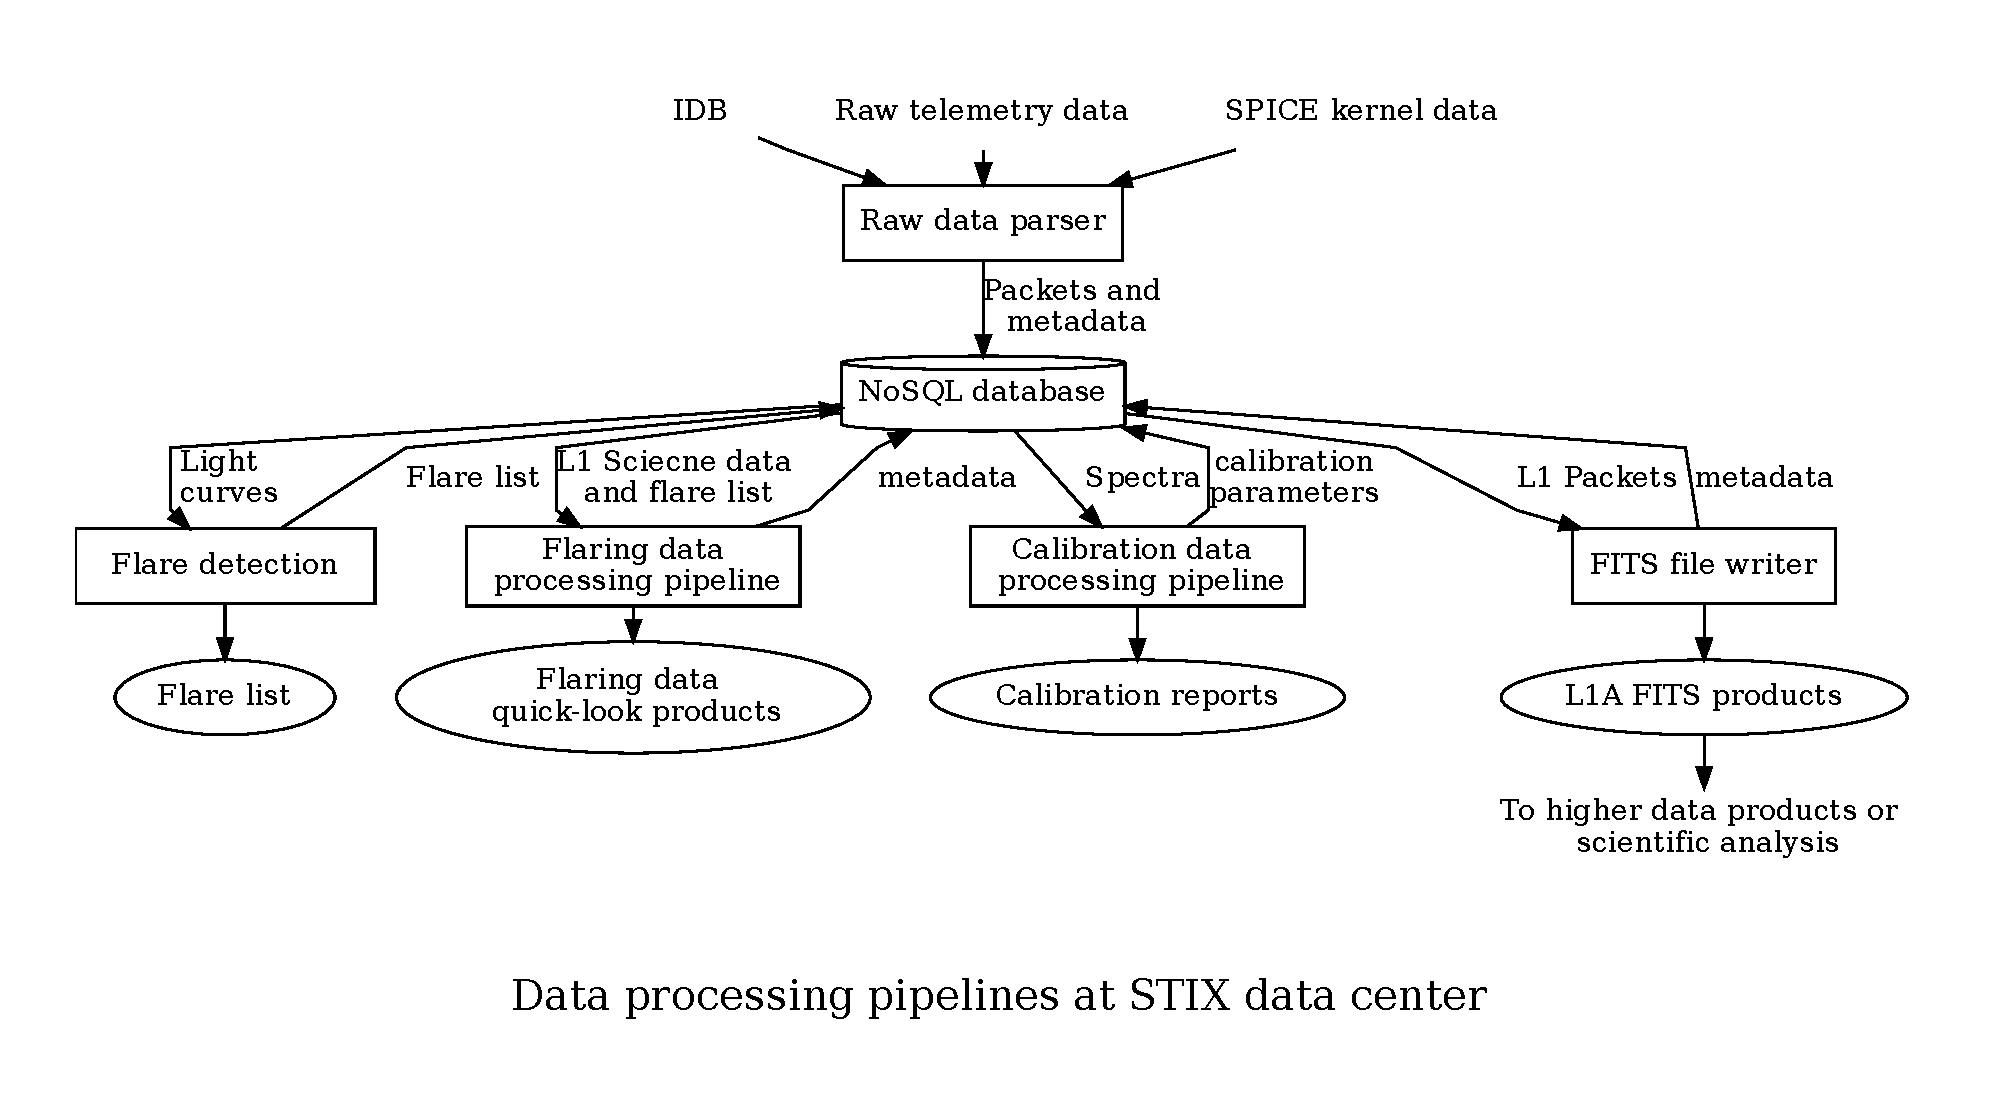
\includegraphics[width=0.9\textwidth]{figures/pipelines.pdf}
    \caption{Data processing pipelines at STIX data center.}
    \label{fig:main_pipelines}
\end{figure*}
The pipelines immediately process the new telemetry data arriving at the STIX data centers, as shown 
in Fig. \ref{fig:main_pipelines}. 
The processing is started with raw packet parsing. The parsed level-1 packets are written to a NoSQL database. Then they are selected  are processed in 4 different paths, 
In the first path,  housekeeping, quick-look and science packets are successively selected and used to create L1-A FITS files, 
which can be used for scientific analysis. The second path selects calibration data from the database and extracts energy calibration factors for instrument monitoring. In the third path, quick-look packets are selected and used to identify solar
flares; The fourth path processes flaring data, generating higher data products.   

\subsection{Raw data parsing and database}
New telemetry data arrived at the STIX data center and is immediately processed by the STIX data parser, which is capable of parsing all types of binary telecommands and telemetry packets.   The parsing of packets is based on the mission interface database (MIB), which 
contains information on packet parameters such as names, descriptions, lengths, and
data types. The parser extracts the header and parameters for each raw binary packet
using the information in the MIB.
Packets after parsing contain raw values of parameters. 
 Spacecraft clock times are further converted to UTC times using 
the latest version of SPICE kernel data (\cite{spice1996,spice2018}), compressed integers are  
decompressed by using an energy look-up table and 
housekeeping raw values are converted to 
human-readable values using the calibration factors or look-up tables stored in the MIB. 
Packets after the above processing steps are called level-1 packets. They
have tree structures, each containing two nodes “header” and “parameters”;
the former contains the basic information  of the packet such as timestamp, packet type,
and the latter contains names, 
raw values, engineering values (or decompressed integers) and child nodes of a list of parameters.
Level-1 packets are written 
to a NoSQL database. 
NoSQL database is schemaless,  making it ideal for storing data with complex
structures but small sizes, like STIX level-1 packets.  
NoSQL is also 

In addition to packets, the NoSQL also stores other data extracted by the parser during the parsing of packets, 
for example, 
\begin{itemize}
  \item Raw file metadata. It contains the filename, reception time, observation start time and stops time, MIB and SPICE kernels used by the parser ; 
  \item Bulk science metadata, which contains the observation time range, detector and pixels masks, energy ranges, 
   bulk science data types, and IDs of packets in the database; 
  \item Quick-look light curves.  The dataset contains data on counts, time range, and energy bins extracted from QL LC packets, 
     allowing for quick access to QL data with web pages or APIs;
  \item STIX instrument configurations. 
  It contains the instrument configuration parameters for such as energy conversion factors and ASICs, 
  allowing fast tracking of the instrument settings;
\end{itemize}
Information is necessary for subsequent processing. The
the database is accessible through web pages at the STIX data center website or python APIs. 
\subsection{Data products}
\subsubsection{Level-1 FITS files}
After each new raw telemetry file is parsed, housekeeping, quick look, and science packets  
are selected from the NoSQL database 
and checked for data integrity and consistency. 
Then packets of the same type are merged for the creation of the pre-release of 
level-1 data products (Level-1A) 
 in the FITS format (\cite{fits}), 
which is a portable file standard widely used in the astronomy 
community to store images and tables.
It should be noted that the data levels mentioned here are data processing levels. 
In order not to confuse two conventions, we use different notations to indicate onboard level in this paper. 
Metadata such as observation time range, creation time, filenames, and checksum are written to 
the primary header data units (HDU) of fits files. 
They are also written to a dataset in the database.

Level-1A FITS files are generated automatically and available at the STIX data center within minutes 
after the reception of a raw file.
It should be noticed that predicted SPICE kernels may be used when the reconstructed spice kernels  
are not available, and the L1A data are subjected to some known issues 
due to bugs in the early version of the flight software.
After all the resources are validated,  Level-1  FITS files are created again. 
Level-1  FITS products have almost the same data structures as Level-1A.
\subsubsection{Level-2 FITS files}
Level-1 FITS files are further processed. 
Dead time  correction and energy, make up the second
\subsubsection{Level-3 data products}
Level-3 data products are visibilities and images

\subsection{Energy calibration}
Energies deposited by x-rays are converted from ADC units 
to keV onboard by using an energy look-up table (ELUT),
 which is regularly updated with telecommands.
ELUTs can be constructed using energy conversion factors obtained by determining 
positions of photo peaks in the calibration spectra measured for the onboard Ba$^{133}$ sources.  
As energy conversion factors may change with temperature 
or polarization effects,  calibration spectra need to be analyzed promptly on the ground. 

\begin{figure}
 \centering
  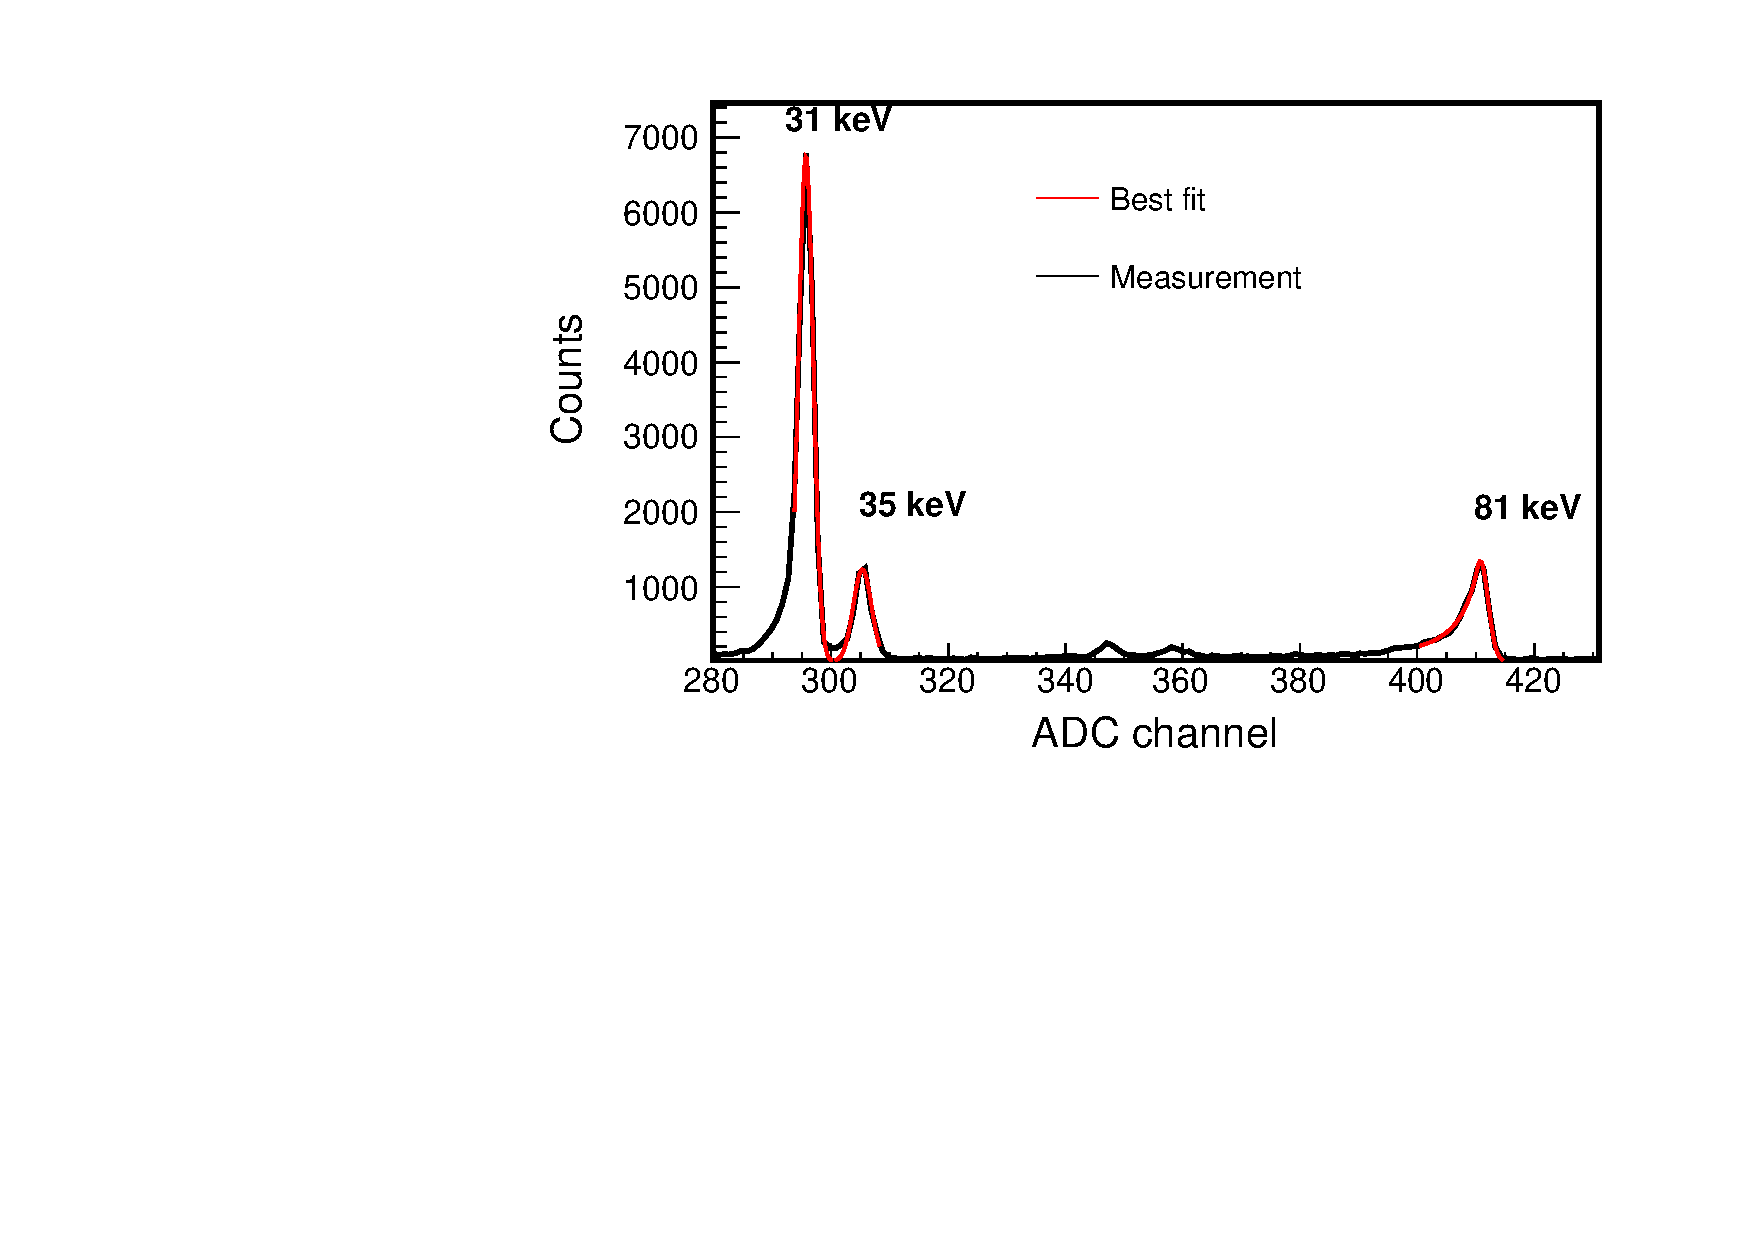
\includegraphics[width=0.8\linewidth]{figures/cal-fit.pdf}
  \caption{An example of STIX in-flight calibration count spectrum.
  The three strongest lines, from left to right, are from 31 keV, 35 keV, and 81 keV
  photons. The first two peaks are fitted by the double-Gaussian function and the high energy peak by  
  the crystal-ball function. }
    \label{fig:cal-fit}
\end{figure}
The right panel of Fig.~\ref{fig:cal-fit} shows 
an example of STIX count spectrum from the in-flight calibration run.  
The three strongest lines are from 31 keV, 35 keV and 81 keV photons. 
The first two peaks are fitted with the double-Gaussian function and the third peak
by the crystal-ball function (\cite{crsystallball}),  which consists of a Gaussian core portion 
and a power-law low-end tail, below a certain threshold.
Then a linear line is fitted to the relation between
the three fitted peak positions (in ADC unit) and the photon energies in units of keV.  
The interception and slope indicate the baseline and gain of the channel. 
The results were compared to those determined using the ECC method (see \cite{ecc,ecc2})), 
 which were found to be consistent within errors.
The above steps are performed for each calibration run automatically 
once the data is available at STIX data center.  The results are written to a
 dataset in the NoSQL database.  It is accessible through a web page at STIX data center or python APIs.

Calibration factors are monitored continuously. Once significant changes are 
observed from those used for the construction of  the onboard ELUT, 
 a new ELUT is created and then uploaded to STIX after being validated by the operations team. 

\subsection{Solar flare identification}
The in-flight software identifies solar flares by comparing  the count rate of 
the background detector with that of other detectors 
 and packs the results into the QL flare flag and location reports.
However,  the reports only provide limited information on flares due to the constraints of telemetry 
bandwidth and the limitation of onboard computing resources, and micro-flares are not 
reported due to the relatively high trigger threshold.
Using QL light curves, solar flares can be identified on the ground in great detail.

QL light curves of the energy range from  4 to 10 keV are used for solar flare identification
on the ground. Identification is based on the fact 
that the background event rate in that energy range is almost constant 
over a timescale of days during quiet sun periods. 
The procedure includes the following steps:
\begin{itemize}
  \item Light curve smoothing. The selected light curve is filtered using an unweighted
  moving average filter with a time window of 1 minute to smooth out statistical fluctuations and electric surge spikes;
  \item “Background” subtraction.  
   A flare may last hours and may have short-duration pulses lying on the main pulse in the light curve.
   The main pulse can be considered as the “background” of those short-duration pulses.
  To identify those short-duration pulses and estimate their durations, 
  we estimate the “background”  using the Statistic-sensitive Non-linear Iterative Peak-clipping algorithm \cite{sinp}, which is widely used in X-ray spectroscopy.
    Then it is subtracted from the smoothed light curve.
  \item Identification of flare peaks. Peaks with counts exceeding a threshold of $2\sigma$ 
  above the quiet Sun background count rates,  
   are selected. The duration of a peak is given by the time difference between the first 
   crossing of the threshold on the left and right sides of the peak;  
  \item Merging of flare peaks. If the time difference between the two consecutive peaks is less than 5 minutes,
   they are considered to be from the same flare.
\end{itemize}

\begin{figure}
  \centering
  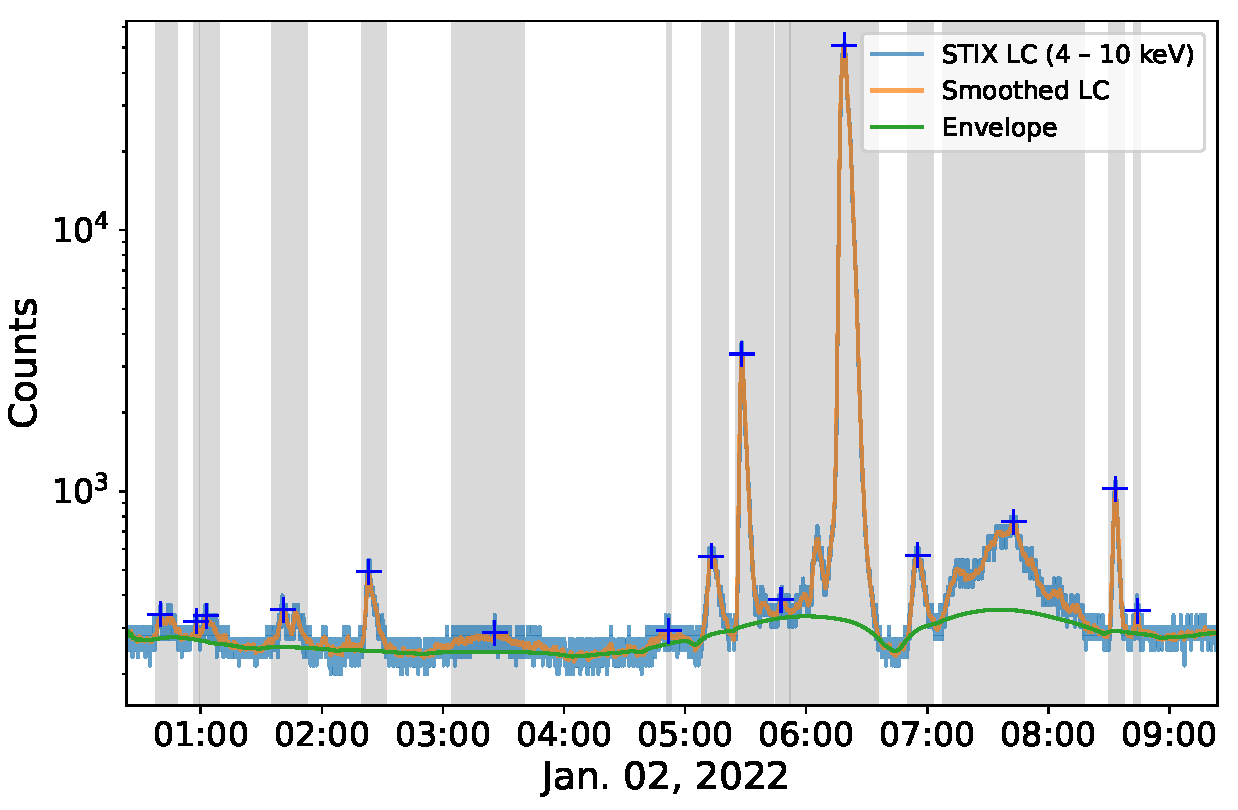
\includegraphics[width=0.8\linewidth]{figures/flaredet.pdf}
  \caption{STIX 4 -- 10 keV QL light curve recorded from 2022-08-10T21:00:00Z to 2022-08-10T18:00:00Z and 
  identified flares.   
  The light curve was smoothed using a moving average filter with a time window
  of 1 minute. 
  The identified peaks are marked with plus signs, and flare time ranges are colored in cyan.
  }
  \label{fig:flare-det}
\end{figure}
As an example, Fig.~\ref{fig:flare-det} shows  the 4 -- 10 keV QL  light curve recorded from 
2022-08-10T10:00:00Z to 2022-08-10T18:00:00Z,
 as well as the smoothed light curve and identified solar flares (marked with plus signs).

For each identified solar flare,  start time, end time, peak time, and peak 
counts are extracted from the selected light curve and assigned 
an 8-digit identification number of the format {\it yymmddHHMM}, which represents the solar flare peak time. 
For example, the identification number 2201010000  indicates that 
the solar flare peak time is at 2022-01-01T00:00:00 UT. 
The above steps are repeated for the QL light curves of the other four higher energies
in the same time frame. This can provide information on the upper limit of the X-ray energy produced by the flare,
which is used to optimize the selection of scientific data to be downloaded. 
Then all extracted information as well as the ephemeris data calculated for the peak time are 
written to a dataset called solar flare list in the NoSQL database.
The flare list database can be queried using a web interface or stixpy.
\subsection{Estimation of background level}
As mentioned earlier, a threshold value calculated using background data needs to be provided when
performing flare identification.  
The background, although stable within a few days, can change over long periods,
 a suitable threshold is important for the accuracy of the identification. 
 Therefore, QL light curves for quiet sun periods are selected by excluding flaring periods. 
 Then median values and variances are calculated from the selected light curves and 
 written to a dataset in the database. They are used as inputs for the next flare identification. 
 Those processing steps are performed automatically after flare identification.

\subsection{Solar flare data analysis pipeline}
\subsubsection{Flare GOES class determination}
\begin{figure}
  \centering
  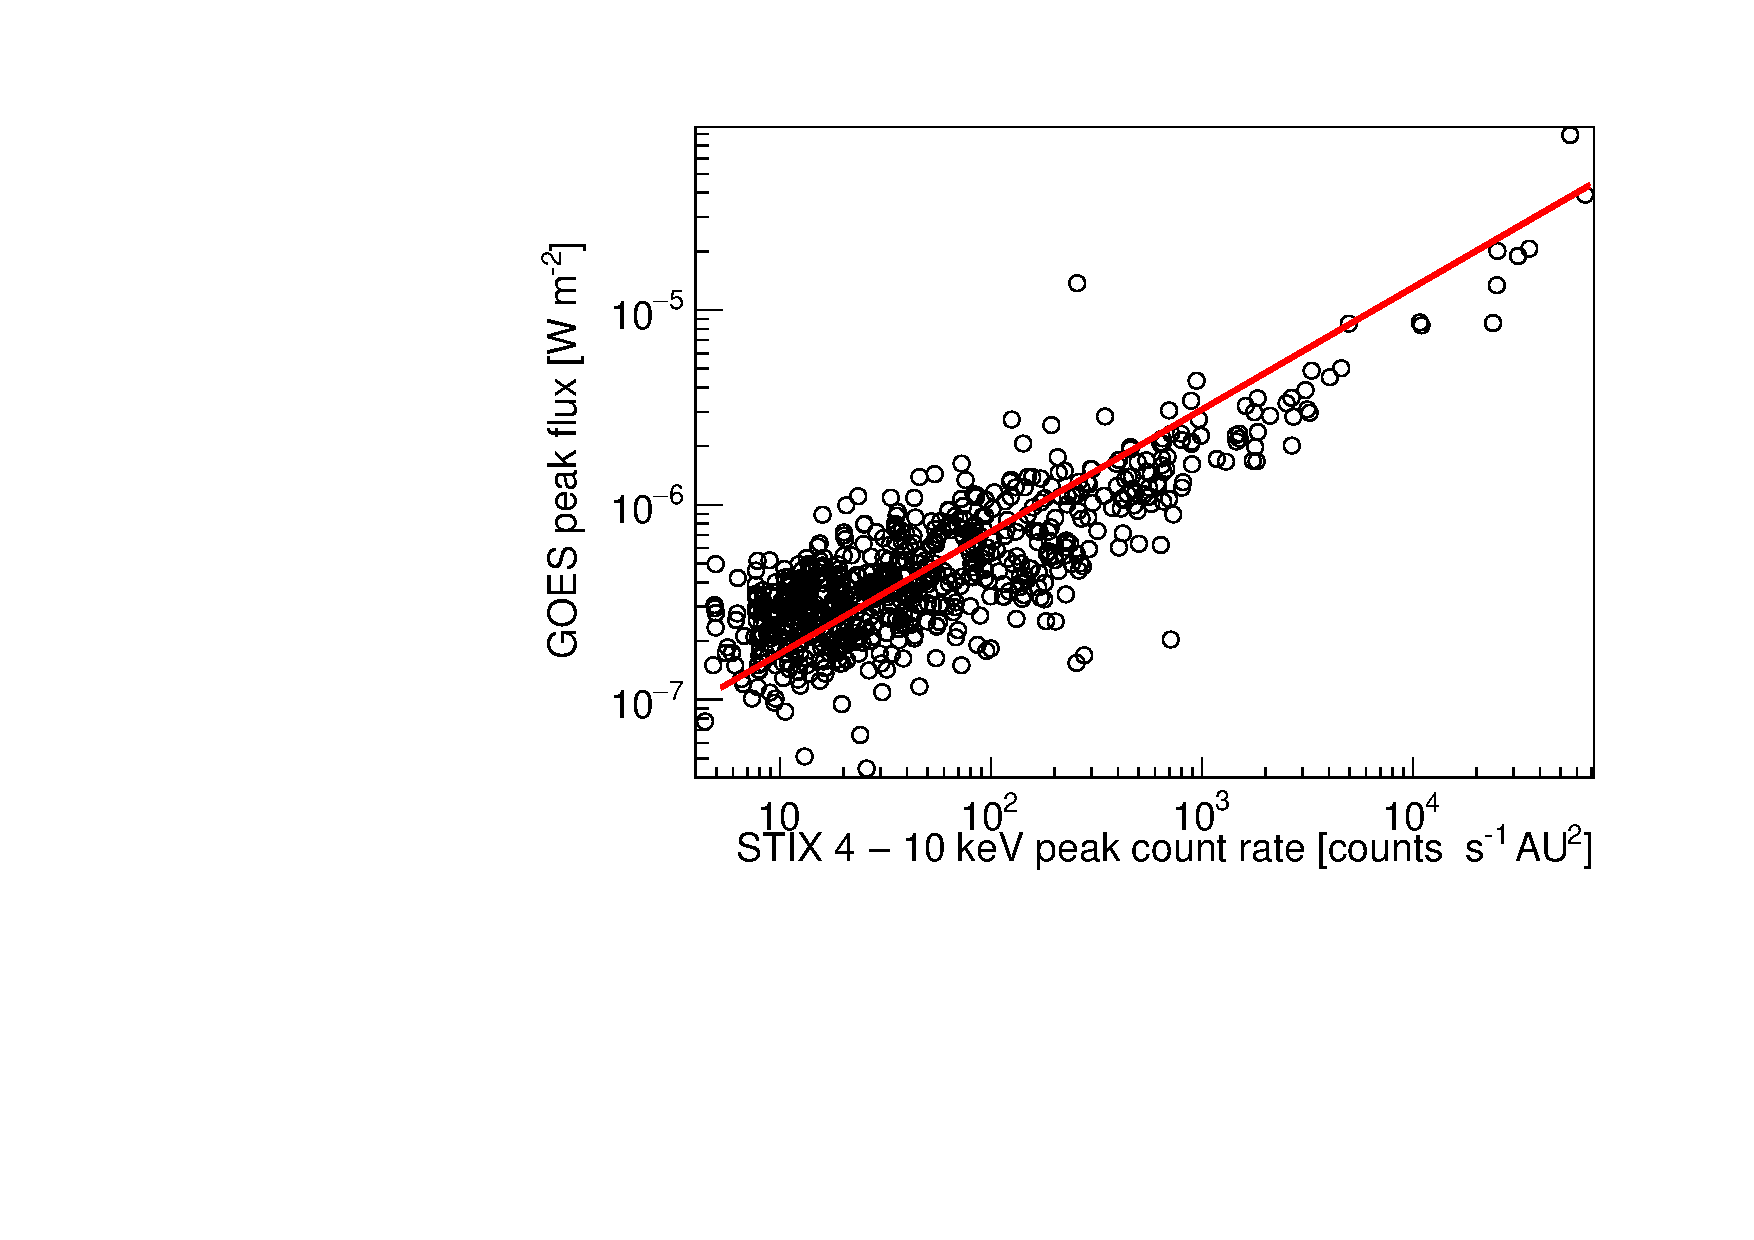
\includegraphics[width=0.8\linewidth]{figures/goes_stix_flux_paper.pdf}
  \caption{Scatter plot of GOES low channel peak flux with respect to STIX 1-AU equivalent  peak count rate in the 4 -- 10 keV range
  for 717 solar flares observed by both GOES and STIX duration of the commissioning phase. 
  The solid line is a linear fit to the log-log graph. 
From the fit, we obtained 
the GOES flux (in units of W/m$^2$) $f = 10^{0.622 -7.376 \log_{10} (X^{'})}$,
where $X^{'}$ is STIX peak count rate corrected for the distance variations between the Sun and Solar Orbiter. 
}
\label{fig:goes-stix}
\end{figure}
It is straightforward to calculate the GOES
class of a flare observed by STIX from GOES flux if it is observed by GOES. 
However,  most of the time, Solar Orbiter is far away from Earth and looks at 
the sun from different angles. Therefore, a considerable number of flares observed by STIX
 are not observed by near-earth satellites (and vice versa). 
As already discussed in Ref.~\cite{andrea2021}, 
it is possible to estimate GOES classes by using STIX count rates.
To study the correction, we selected 717 solar flares observed by 
both GOES  and   STIX during the commissioning phase.   
Fig.~\ref{fig:goes-stix} shows the scatter plot of GOES low channel peak flux with respect to 
STIX peak count rate of the 4 -- 10 keV QL light curves. 
STIX count rates  have been subtracted for background and corrected for 
the difference distance of Solar Orbiter to the Sun using $X^{'}=x r^2$, where $X$ is the count rate after background subtraction
 and $r$ is the distance between the Solar Orbiter and the Sun in units of AU. 
As can be seen in the figure, there is a clear correlation between
these two quantities.  The widespread at the low flux could be explained by the difference in 
the energy response of the two instruments and the flare temperatures. 
A linear line was fitted to the correlation in the log-log scale. 
From the fit, we obtained 
the GOES flux in units of W/m$^2$ $\log_{10}(f) = 0.622 -7.376 \log_{10} (X^{'})$.
%where $x^{'}$ is STIX
%peak count rate corrected for the distance variations between the Sun and Solar Orbiter. 
The formula is currently used to estimate GOES classes of flares observed by STIX. 
It is worthwhile to mention that more observations will be included in the fit.
The estimated GOES class as well as those from GOES measurements 
are stored in the flare list database. 

\subsubsection{Coarse flare location estimation}
Flare centroid location can constrain the flaring region when reconstructing flare images.
STIX uses a dedicated sub-collimator called Coarse Flare Locator (CFL) to estimate flare locations.
The CFL consists of a front grid with
a distinctive pattern that selectively illuminates pixels of a 
dedicated detector based on the source location.
Flare location is estimated onboard by maximizing the correlation between observed CFL pixel counts 
with expected counts using a look-up table. 
However, due to the constraints of onboard computation, the onboard flare location is  only calculated for intermediate flares 
and has an accuracy of about 2 arcmin. 
With the downloaded measured counts in each pixel,
the coarse flare location can be reconstructed on the ground as well. 
This allows for more sophisticated algorithms, greater flexibility in selecting time and energy 
range to be integrated, and more careful background subtraction.

\begin{figure*}
  \centering
  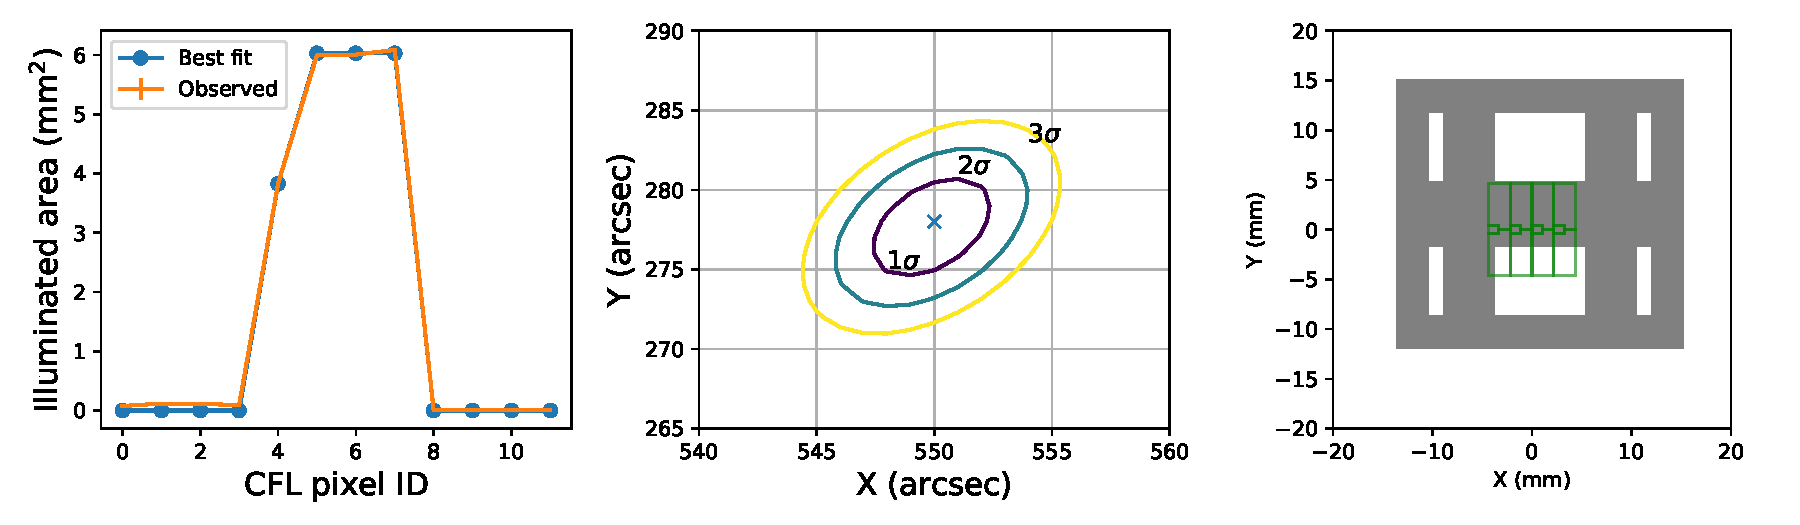
\includegraphics[width=0.95\linewidth]{figures/cflMay07.pdf}
  \caption{
   Left: Areas of illuminated regions of 12 pixels calculated by combining
  the twelve pixels counts with averages from other detectors, and the best fit. 
  Pixels 0 to 3 are the top big pixels, Pixels 4 to 7 are the bottom pixels, and 8 to 11 are the small pixels as shown in the right panel.
   Middle: Best-fit flare centroid location (marked by x) and its 1$\sigma$, 2$\sigma$, and 3$\sigma$ confidence contours.
   The best-fit location is obtained at (550, 278) sec. 
    Right:  Shadow (the gray shaded regions) of CFL sub-collimator projected on the detector 
  for the best-fit flare location. }
  \label{fig:cfl}
\end{figure*}

The coarse location of an observed flare is estimated on the ground after its pixel data (onboard level-1) is parsed.
The procedure consists of the following steps:
\begin{itemize}
  \item Selection of pixel data based on the flare time range and energy range information stored in the flare list dataset;
  \item Subtraction of background. The most recent level-1 dataset for the quiet sun period is used for background subtraction;
  \item Calculation of the mean fluence except for the CFL and the background detectors; 
      Except for those two detectors, the ratio between the illuminated area and total area $r$ only depends on the 
      slit width and the pitch width. It doesn't vary with the position of the flare in the STIX field of view (FOV).  
      Therefore, the fluence of a detector can be given by $F=c/(r S_{\mathrm(d)})$,  where $c$ is the registered 
      count and $S_\textrm{det}$ the sum of the sensitive areas of twelve pixels. 
  \item Calculation of the areas of illuminated regions on CFL pixels $\vec{S}$ using $\vec{S} = \vec{C}/F$, where $C$  is an array of counts 
  recorded by 12 pixels. Their errors in the areas are also calculated; 
  \item  Coarse flare location is estimated by minimizing the weighted sum of squared deviations 
  (i.e. weighted chi-squares) between the calculated illuminated areas and expectations
  simulated for potential flare locations in a 400 $\times$ 400 grid, whose locations are separated by 10 arcsec.  
  \item Saving the calculated flare location to the flare list dataset. 
\end{itemize}
As an example, the left panel of Fig.~\ref{fig:cfl} shows the calculated and best-fit illuminated areas 
of the CFL pixels measure observed for STIX flare 2105071900 (GOES class M3.9);   the middle panel shows the best-fit 
flare centroid location, as well as its $1\sigma$, $2\sigma$ and $3\sigma$ contours. 
The simulated shadow of the CFL sub-collimator is shown in the right panel. 
%\subsubsection{Joint observation}

\subsubsection{Image reconstruction and spectral analysis}
\begin{figure*}
  \centering
  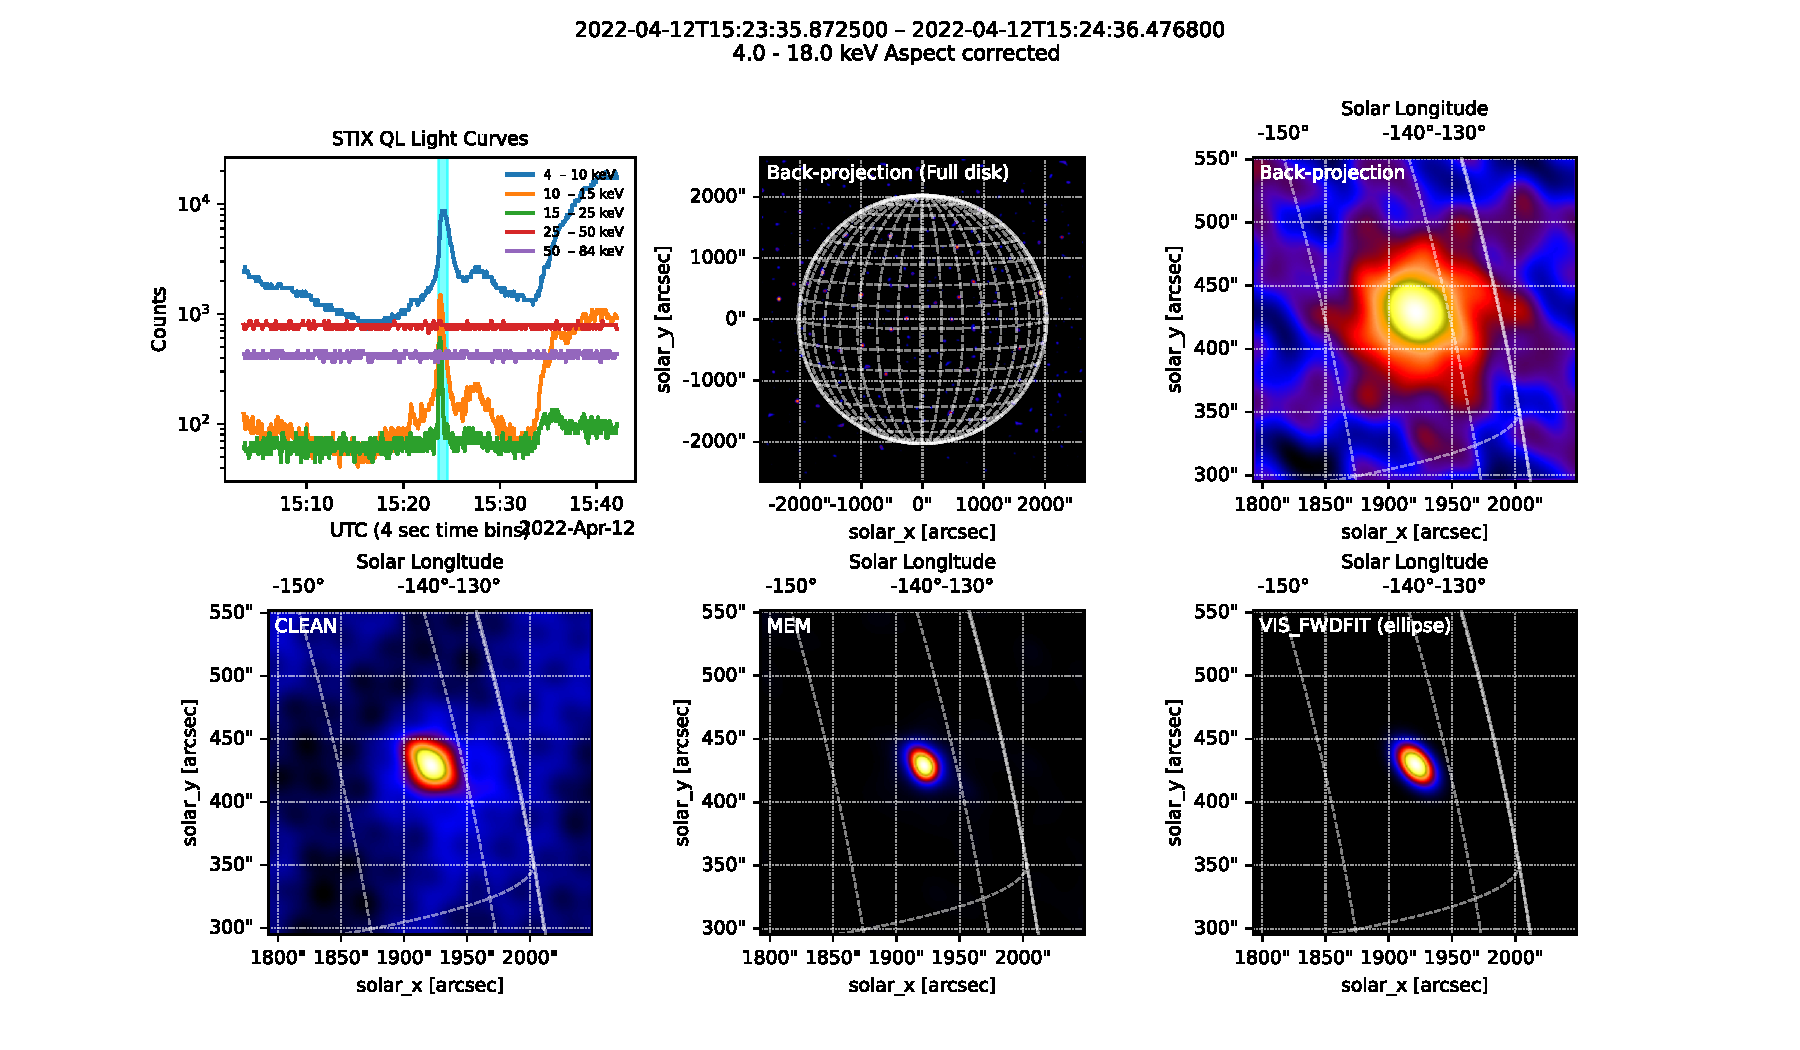
\includegraphics[width=0.95\linewidth]{figures/imaging_pipeline.pdf}
  \caption{ 
   STIX Quick-look light curves and reconstructed images of the solar flare observed at 2022-03-08T08:55:17Z, 
   created by the image reconstruction pipeline.  The period at the peak was selected and 
   Back-projection, CLEAN, EM, and VIS\_FWDFIT
    algorithms were used for reconstructing images. Image products are accessible
   at STIX data center.}
  \label{fig:imaging}
\end{figure*}
STIX detects thousands of solar flares each year. However, only
 a part of them is analyzed in detail by solar physicists. 
To facilitate the selection of flares of interest, a flare imaging reconstruction and the spectral fitting pipeline 
has been developed and integrated into the main data processing pipeline on the platform. 
For each flare, pixel counts recorded within a one-minute time frame around the flare peaks  
are selected.
Reconstruction of an image requires inputs such as background data in the same level, 
STIX pointing information, spacecraft orientation. 
They are prepared based on the knowledge of NoSQL. 
After background subtraction, transmission, and dead time corrections, the selected counts are used for 
the calculation of visibilities for two energy ranges 4 -- 10 keV (thermal emission) and 16 -- 28 (non-thermal)  
keV.
Then images are reconstructed with four different algorithms: Back-projection, CLEAN, 
MEM and VIS\_FWDFIT \cite{paolo2020,clean, mem}.
Reconstructed images are further corrected for STIX off-pointing and spacecraft rotations with the auxiliary data. 
As an example,  the first panel of Fig. ~\ref{fig:imaging} shows 
the light curves and time range selected for a flare that occurred at about 2022-03-08T08:55:17Z.
The rest of the panels show the reconstructed images. 
The final by the pipeline are written to files in FITS  and PNG formats, while
their metadata are written to the NoSQL database.  
%They are accessible from STIX data center website or via stixdcpy\footnote{stixdcpy}.
\subsubsection{Spectral analysis}
Energy spectra provide direct information on electron acceleration in solar flares. 
The x-ray spectral fitting package OSPEX in SSWIDL includes a wide range of commonly used 
functions for parametrizing the thermal
and non-thermal components, as well as an interface to perform
the fits \footnote{\url{https://hesperia.gsfc.nasa.gov/ssw/packages/spex/doc/}}.
It reads pixel count data from L1 FITS files, corrections for dead time, transmission 
and energy binning for the counts,  
and calls  OSPEX routines for spectral fitting. 
\begin{figure}[h]
  \centering
  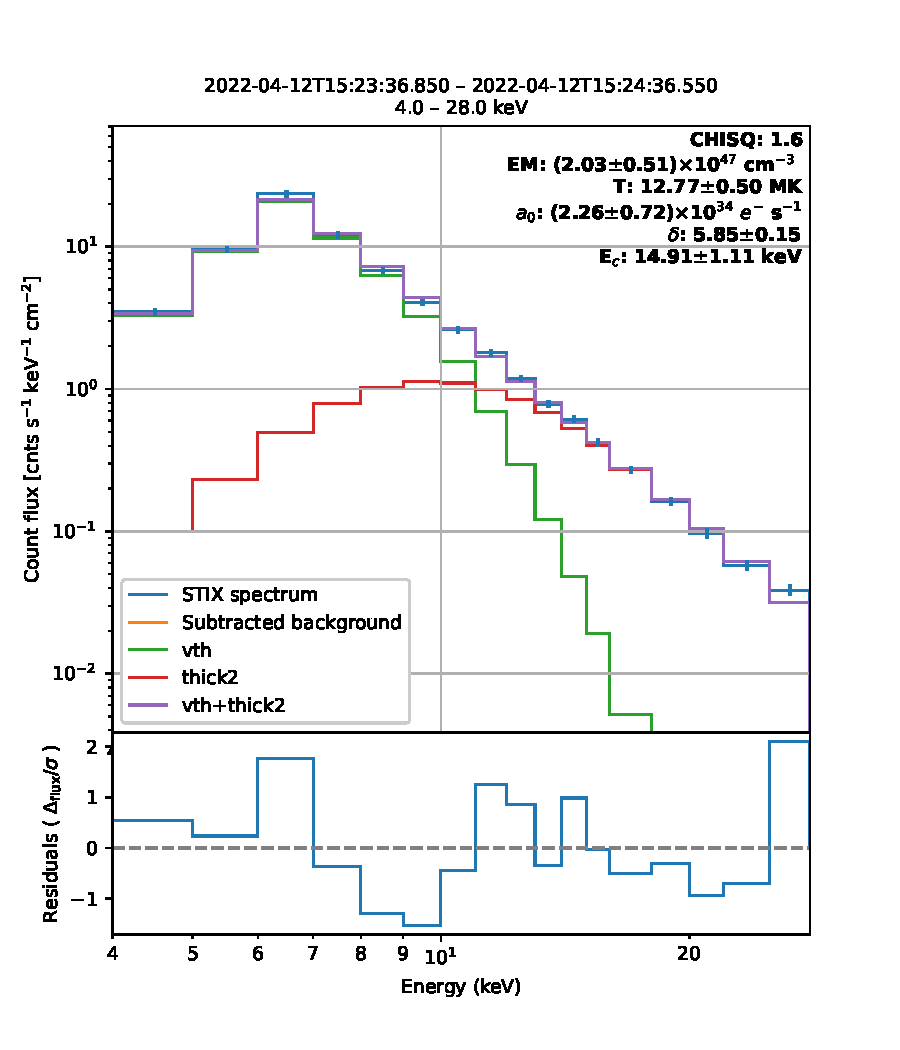
\includegraphics[width=0.9\linewidth]{figures/ospex.pdf}
  \caption{ 
    An example of spectral fitting results. The imaging and spectroscopy pipeline performs
    spectral analysis for all flares in the flare list. Spectral fitting results are written to both FITS files and 
    the NoSQL database.
   }
  \label{fig:ospex}
\end{figure}
\section{Science data request strategy}
As mentioned earlier, STIX only down-links low-latency data 
automatically due to the data rate constraints.  
Pixel data with higher time and energy resolution contain much richer information. 
They persist in the onboard archive memory for about five to six months 
before they are overwritten.
They can be compressed and 
down-linked after receiving data request telecommands initiated by the STIX operation team. 
A data request telecommand needs to provide information on the
time range, minimal time binning, energy range, energy binning  and selected detectors (or pixels), based on 
the knowledge from low-latency quick-look light curves.
Requesting science data from STIX is a tedious task, as it must take
into account many factors, such as constraints on the  allocated telemetry data rate, 
the daily maximum number of requests that can be submitted,  
the onboard time binning, 
solar flare fluxes and the scientific value of the data. 
After two years of operation, the following data selection strategy has been adopted: 
\begin{itemize}
  \item 
  Level-1 pixel data 
  of the flaring period is requested for detected flares with a total number of signal counts  greater than 1000, 
  which is the minimum count to reconstruct an image.  
  To minimize the telemetry data size, 
  the energy range of the request is limited to the range with signal counts based on the 
  knowledge from light curves. 
  If the pixel-summed peak count rate is less than 125 counts/sec
  (equivalent to the count rate observed for a B3 flare at 1 au), 
  a single time-bin is requested. Otherwise, a finer time resolution of science data is requested.
  The actual time resolution is adjusted based on the amount of data allocated.
 \item Spectrograms (onboard level-4) require a relatively small amount of data, therefore
  the highest possible time resolution (\~ 0.5 seconds depending on the configuration)
   and energy resolution  (no rebinning of science energy bins) are requested for all periods that STIX is in NOMINAL mode. 
\item At least one level 1 scientific data background data is requested per day. 
Background period selection is done by excluding periods from the list of flares stored in the database. 
If a quiet solar period is not found, a relatively quiet solar period will be selected. 
To reduce the amount of telemetry data, 
background data request counts are time-integrated over the requested period, i.e., a single time-bin.
\end{itemize}
A routine has been developed to create the data requests mentioned above automatically. 
A unique ID is assigned to each request.
Unique IDs have a format of {\em yymmddxxxx}, where 
the first eight digits indicate the two-digit year,  month, and day of the data start time, respectively, 
and the last four digits are a random number, which is unique for the day.  
Information of created data requests is stored in the NoSQL database. 
After being checked by STIX team, data requests are flagged as pending requests.
Then they are selected and compiled into instrument operation requests (IORs), which are used to create the final telecommands
to be executed by the instrument.
Apart from those automatically created data requests, 
data requests are also created by the instrument team for special requirements.
\section{STIX data platform user interfaces}


\subsection{Interactive web pages}
\begin{figure}[h]
  \centering
  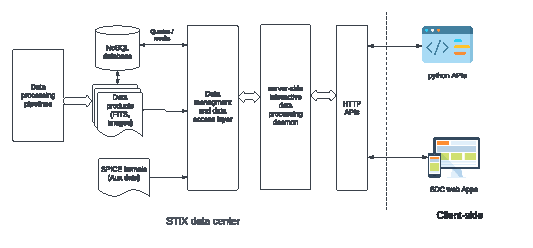
\includegraphics[width=0.9\linewidth]{figures/interfaces.pdf}
  \caption{ 
    Data flow at STIX data center.
  }
  \label{fig:interfaces}
\end{figure}

\begin{figure*}[h]
  \centering
  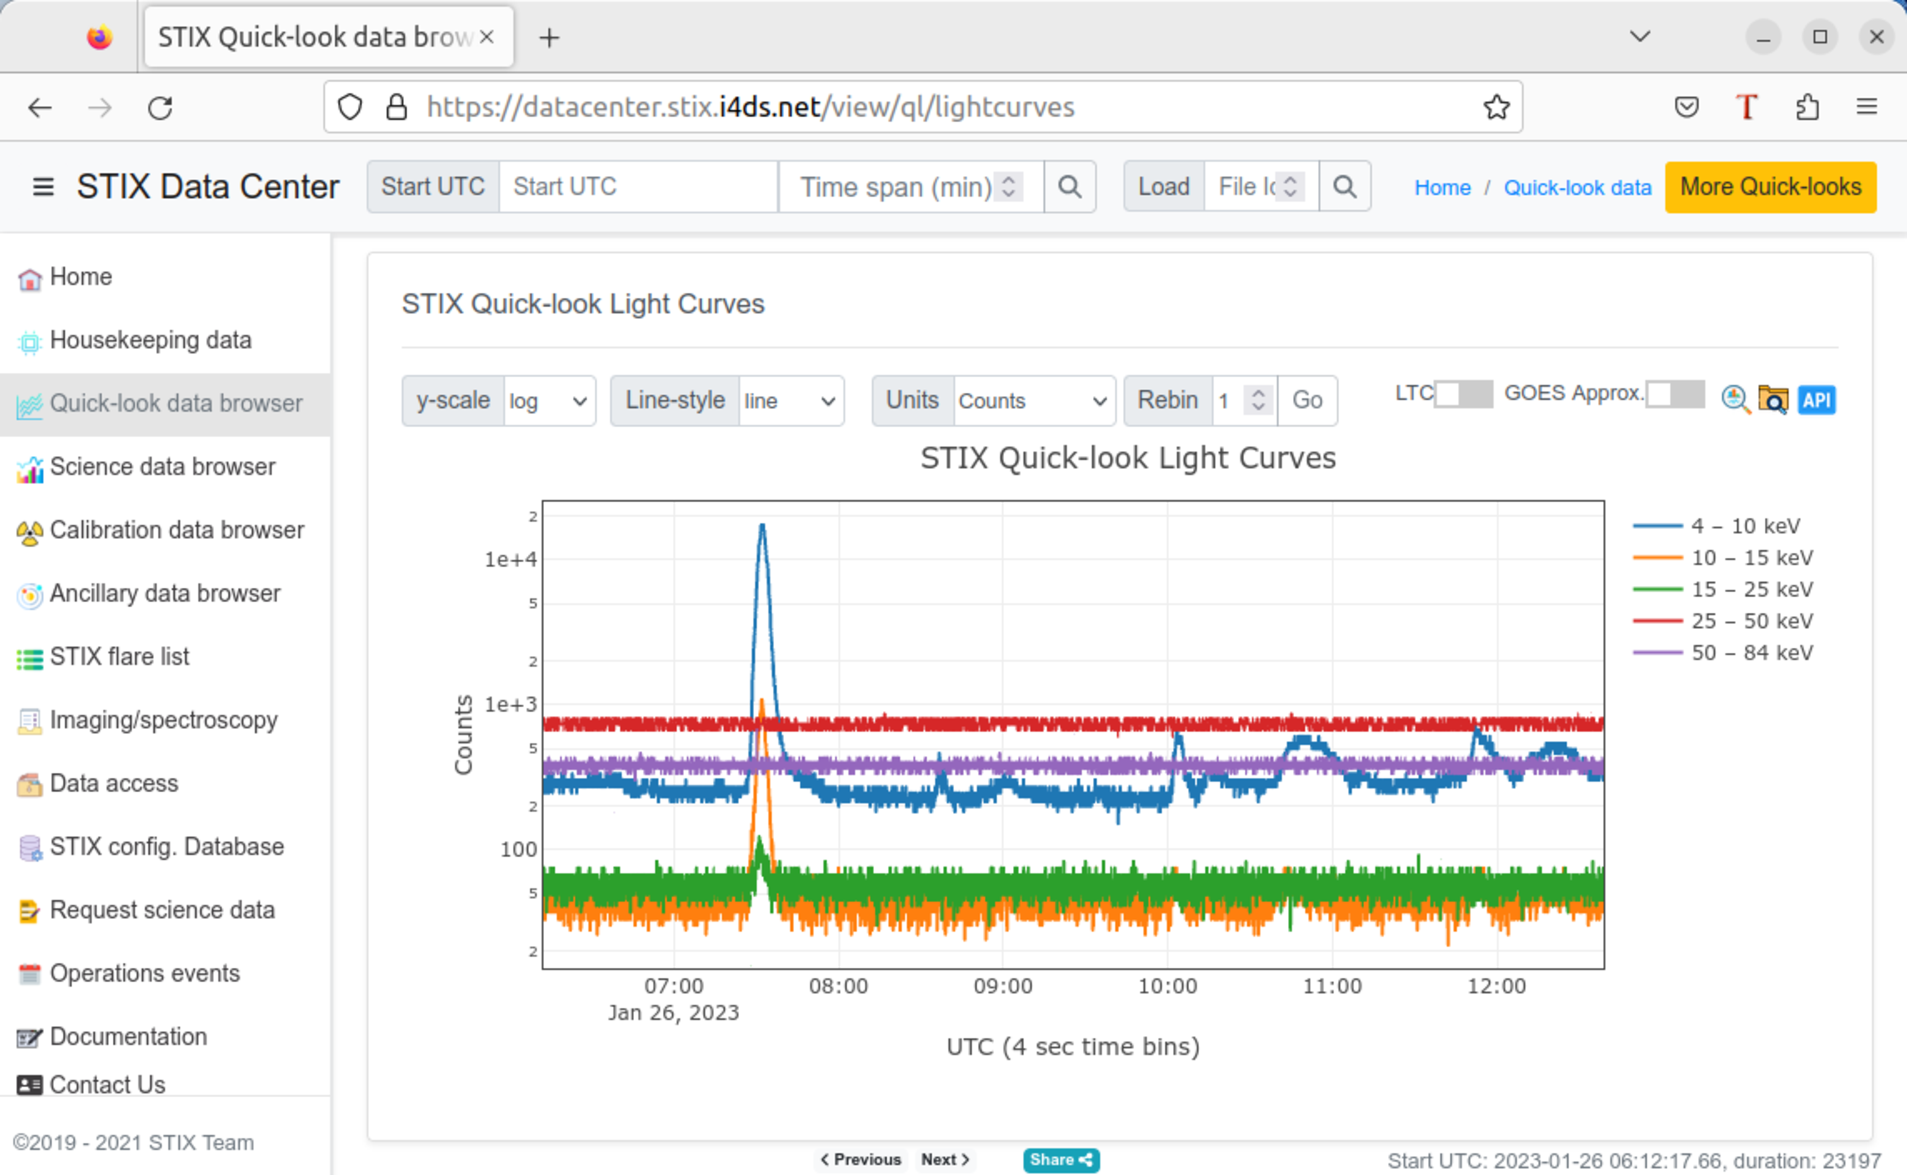
\includegraphics[width=0.7\linewidth]{figures/data-browser.pdf}
  \caption{ 
    Interactive web-based STIX Quick-look data browser. 
    Apart from STIX Quick-looks, it can also display quick-looks of simultaneous measurements 
    performed by other instruments, such as GOES X-ray fluxes, SDO/AIA images and Solar Orbiter EUI. 
    The browser is available at the link \url{https://datacenter.stix.i4ds.net/view/ql/lightcurves}.}
  \label{fig:qlbrowser}
\end{figure*}


To facilitate access to the data, a series of web APIs have been developed.
The web APIs accept HTTP requests from the client side, 
then the requests are processed on the server-side
 and the results are returned to the client side.  
The web APIs provide access to all STIX data products 
and the metadata stored in the NoSQL database. 

Based on the web APIs, we have built dozens of different web applications to manage and visualize 
different data products. 
The reason that we chose web techniques for the data browsers is that
web applications provide many advantages, such as clear cross-platform usability, 
wide access with browsers, allowing rapid development and easy maintenance. 

As an example, 
Fig.~\ref{fig:qlbrowser} shows a screenshot of the interactive web-based STIX Quick-look data browser hosted 
at STIX data center website.  It allows users to browse any historical STIX Quick-look data.
On the browser, users can specify time ranges of Quick-look data to be loaded.
After the web API on the server receives a request, 
it reads level-1 packets from the NoSQL database measured in the given time frame, and sends the
compiled and serialized data back to the web browser. 
Then the data are parsed and used to create an interactive light curve plot on the client side by using JavaScript.
Thanks to the use of state-of-art web technologies, the interactive plot allows users  
to rebin integration times, correct light travel times, estimate GOES fluxes and export data to local files. 
Apart from STIX quick-looks, quick-looks of 
simultaneous measurements performed by other Sun observing instruments
can also be loaded on the same page, which greatly facilitates finding of the 
events of interest for joint analysis. 

Based on similar concepts, tens of web tools have been developed for 
browsing other STIX data products. 
The four most used by STIX data users are: 
\begin{itemize}
  \item  Science data browsing and interactive analysis tool:
  It provides users tools to search for science data, 
  download science data, 
  perform common data analysis tasks and visualize science data and
  data analysis results. 
  On the web app, users can also select data of interest  
  for common analysis tasks, such as background subtraction, energy and time rebinning, 
  and estimation of coarse flare locations, which are on the client side using JavaScript.
Moreover, Users can also submit imaging and spectroscopy requests to the cloud with the
 interactive analysis tools on the page without the need of installing software. 
 Interactive plots are created using the results. Users can also export data from the interactive plots or 
  download the science data in the FITS format to the local disk for further analysis. 
  The browser greatly reduces the barrier to explore STIX science data for newcomers and also 
  for experienced users. 

  \item  Preview images and spectroscopy product browser:
  The tool provides a web-based imaging and spectroscopy manager. With the tool, users can view the 
  reconstructed solar flare images and fitting results from 
  automated imaging/spectroscopy runs and those submitted by register users. 
  It also allows users to plot the time evolution of emission measures and temperatures, as well as animation of x-ray images 
  for the selected runs.  Users can also create IDL or python templates, allowing the same results to be reproduced on their local machine.


  \item  Auxiliary data viewer: 
  The auxiliary data viewer allows users to view any historical auxiliary data of Solar Orbiter. 
  After receiving the time range information from the client-side,
  the server-side uses the SPICE kernels and SPICE toolkit (or STIX aspect solutions when they are available) to calculate 
  auxiliary data commonly used in data analysis for user-selected time ranges, 
  such as spacecraft location, velocity, light time difference, STIX pointing, 
   STIX FOVs, and angles from different observers, and sends the results to the client side. 
   Then the results are charted on the web page using JavaScript. 

  \item  Housekeeping data browser: 
The housekeeping browser allows users to browse any historical HK data from STIX. After the housekeeping browser receives the user's request, it sends the request to the server. The server directly uses the NoSQL data package to scale and serialize the data and return it to the browser. The browser then uses the data to generate interactive graphics (such as sensors). 
temperature, voltage, working status, memory status, etc.).
which provides great convenience for load operation control and for understanding instrument status in data analysis.
\item STIX data access page:  
STIX adopts an open data policy. 
STIX data products are published on the data access page once they are generated. 
On the page, users can search for data products by providing the data type and the observation time range  
, or download data products to local disks for further analysis. 

\end{itemize}




\subsection{STIX data center interface:  stixdcpy}
{\it stixdcpy} is a python package that facilitates access and analysis of STIX data.
It provides APIs to query and download data from STIX data center 
 and a set of tools for visualizing data and performing common analysis tasks. 
 With stixdcpy, users can query and download the following,  almost all data products available at STIX data center. 

similar to the web tools, stixdcpy also provide common data analysis algorithm, such as 
live time correction, transmission correction, data clipping, and  merging, auxiliary data tools, 
creating quick-looks for products 
stixdcpy is still under  development 
The source code of stixdcpy is hosted at the github repo at  \url{https://github.com/i4Ds/stixdcpy}.

\section{Summary}
\label{sec:summary}
STIX is one of ten instruments onboard Solar Orbiter.
 It measures the spectrum and takes X-ray images of solar 
 flares in the energy range 4 -- 150 keV. Solar Orbiter was launched into space on February 10, 2020. 
 During nominal operations, STIX continuously generates telemetry data. 
 To process and archive data as well as to support the operation of 
 instruments and scientific activities using STIX data, 
 automated data processing pipelines and data platforms have been 
 developed for STIX at FHNW. 
 The pipelines generate telemetry at different levels and perform common scientific analyses. 
 The platform provides 
 all STIX data products of different levels and also provides users 
 with various web-based tools to search for,  browser STIX data products. 
 It also provides web-based tools to perform common analysis tasks with STIX data. 
  The data center is designed to work in a 
 fully automatic mode with minimal human intervention. The concept has proven successful 
 and has been running continuously for over two years.
The platform not only facilitates the operations of the instrument but also provides great support to STIX data users.



\bibliographystyle{aa}
\bibliography{citations}

\end{document}